\subsubsection{Concavity}


A function $f:Q^{X}\to Q^{Y}$ is \emph{concave} if for all $\alpha\in [0,1]$, $ x ,  y  \in Q^{X}$ and $b\in Y$ 
$$
f(\alpha\cdot  x +(1-\alpha)\cdot  y  )_{b} \geq \alpha f( x )_{b} + (1-\alpha)f( y  )_{b}
$$



\begin{proposition}
All tropical functions $f: Q^{X}\to Q^{Y}$ are concave.
\end{proposition}
\begin{proof}
Let us first show that all functions of the form $f( x )_{b}= \mu  x + c$ are concave:
we have $f(\alpha x + (1-\alpha) y  )_{b}= \mu(\alpha x )+(1-\alpha) y  )+c=
 \mu(\alpha x )+(1-\alpha) y  )+\alpha c+(1-\alpha)c=
 \alpha(\mu  x  + c)+(1-\alpha)(\mu  y  +c)=\alpha f( x )_{b}+(1-\alpha) f( x )_{b}$.


To conclude, let us show that if $(f_{i})_{i\in I}$ is a family of concave functions from $Q^{X}$ to $Q^{Y}$, the function $f=\inf_{i\in I}f_{i}$ is also concave: we have
$f(\alpha x  +(1-\alpha) y  )_{b}=
\inf_{i\in I}f_{i}(\alpha x +(1-\alpha) y  )_{b} \geq 
\inf_{i\in I}\alpha f_{i}( x )_{b}+(1-\alpha)f_{i}( y  )_{b}
\geq 
\inf_{i\in I}\alpha f_{i}( x )_{b} + \inf_{j\in I}(1-\alpha)f_{j}( y  )_{b}
=
\alpha \cdot (\inf_{i\in I}f_{i}( x )_{b})+ (1-\alpha)\cdot( \inf_{j\in I}f_{j}( y  )_{b})=
\alpha  f( x )_{b}+(1-\alpha)f( y  )_{b}$, where we used the fact that given families $a_{i},b_{i}$ of reals,
$\inf_{i}a_{i}+b_{i}\geq \inf_{i}a_{i}+\inf_{j}b_{j}$.
This follows from the fact that for all $i\in I$, $a_{i}+b_{i}\geq \inf_{i}a_{i}+\inf_{i}b_{i}$.
\end{proof}

%
%
%Concavity is a useful property, as it leads to establish the following:
%\begin{proposition}
%For any tropical function $f: Q^{X}\to Q^{Y}$, 
%\begin{enumerate}
%\item $ \alpha f( x )_{b}\leq  f(\alpha x )_{b}$;
%\item $f( x + y  )_{b}\leq f( x )_{b}+f( y  )_{b}$;
%\item $f( x + y  )_{b} \leq f( x )_{b} + \phi_{\mu,b}( y  )$ 
%for all $\mu\in \C M_{\mathrm{fin}}(X)$.
%
%\item if $ x  <  y   <  z  $, then 
%$$
%\frac{f( y  )-f( x )}{| y  - x |} \leq \frac{f( z  )-f( x )}{| z  - x |}
%\leq \frac{f( z  )-f( y  )}{| z  - y  |}
%$$
%
%\item the function $R_{b}( x ,  y  )= \frac{f( x )_{b}-f( y  )_{b}}{|  x -  y  |}$ is monotonically non-decreasing in $ x $ (for fixed $ y  $) and in $ y  $ (for fixed $ x $).
%
%\end{enumerate}
%\end{proposition}
%\begin{proof}
%Since $f$ is concave, we have that for all $ z  $, 
%$f(\alpha\cdot z  )=f(\alpha\cdot z  +(1-\alpha)\cdot 0)\geq 
%\alpha f( z  )+(1-\alpha)f(0)\geq \alpha f( z  )$. 
%
%For the second one, 
%if $f( x )=\mu  x +c$, then $f( x + y  )= \mu  x + \mu  y   + c  \leq
%\mu  x  + \mu  y   + 2c = f( x )+f( y  )$.
%Moreover, if $(f_{i})_{i\in I}$ is a family of functions such that $f_{i}( x + y  )\leq f_{i}( x )+f_{i}( y  )$, then 
%$f=\inf _{i\in I}f_{i}$ also satisfies this property: 
%one has $f( x + y  )=\inf_{i\in I}f_{i}( x + y  ) \geq \inf_{i} f_{i}( x )+f_{i}( y  ) \geq \inf_{i}f_{i}( x ) + \inf_{i}f_{i}( y  )=f( x )+f( y  )$.
%%Now we can compute
%%\begin{align*}
%%f( x + y  )_{b}& =
%%
%%\end{align*}
%
%The third one follows immediately from the second one, since $f( y  )_{b}\leq \phi_{\mu,b}( y  )$ for all $\mu\in \C M_{\mathrm{fin}}(X)$.
%












%\end{proof}

%\newpage

\subsubsection{Proof of Theorem~\ref{theorem:fepsilon}}

We give below the complete statement of Theorem \ref{theorem:fepsilon} together with its proof.

First, let us set the following:
\begin{definition}
 Let $\preceq$ be the pointwise order on $\N^k$ (i.e.\ for all $ m  , n  \in \N^{K}$, $ m  \preceq  n  $ iff $m_{i}\leq n_{i}$ for all $1\leq i\leq K$).
 Of course $ m  \prec  n  $ holds exactly when $ m  \preceq  n  $ and $m_{i}<n_{i}$ for at least one $1\leq i\leq K$.
 Finally, we set $ m  \prec_{1} n  $  iff
$ m  \prec  n  $ and $\sum_{i=1}^{K}n_{i}-m_{i}=1$ (i.e.\ they differ on exactly one coordinate).
\end{definition}

We will exploit the following:

\begin{remark}\label{rmk:AC}
\text{If $U\subseteq \N^{K}$ is infinite, then $U$ contains an infinite ascending chain $ m  _{0}\prec  m  _{1} \prec  m  _{2} \prec \dots$.}.

This is a consequence of K\"onig Lemma (KL): consider the directed acyclic graph $(U,\prec_{1})$, indeed a $K$-branching tree; if there is no infinite ascending chain $  m  _{0}\prec  m  _{1} \prec  m  _{2} \prec \dots$, then in particular there is no infinite ascending chain $  m  _{0}\prec_{1}  m  _{1} \prec_{1}  m  _{2} \prec_{1} \dots$ so the tree $U$ has no infinite ascending chain; then by KL it is finite, contradicting the assumption. 
\end{remark}

\begin{theorem}[Theorem \ref{theorem:fepsilon}]
Let $f:\overline{\R}_{\geq 0}^{\{1,\dots, K\}} \to \overline{\R}_{\geq 0}$ tropical analytical, with matrix $\hat f : \N^{K} \to \overline{\R}_{\geq 0}$.
Then, for all $0<\epsilon<+\infty$, there is $\mathcal{F}_\epsilon\subseteq\N^{K}$ s.t.\
\begin{enumerate}
 \item $\mathcal{F}_\epsilon$ is finite
 \item If $\mathcal{F}_\epsilon= \emptyset$ then $f( x ) = +\infty$ for all $ x \in \overline{\R}_{\geq 0}^{\{1,\dots, K\}}$
 \item If $f( x _0) = +\infty$ for some $ x _0\in [\epsilon,\infty)^{K}$ then $\mathcal{F}_\epsilon= \emptyset$
 \item The restriction of $f$ to $[\epsilon,+\infty]^{K}$ coincides with the  \emph{tropical polynomial}:
      \[
        P_\epsilon( x )= \min\limits_{ n  \in\mathcal{F}_\epsilon} \set{\hat f ( n  ) +  n   x }.
      \]
      where $ n   x = \sum_{i=1}^{K}n_{i}x_{i}$.
\end{enumerate}
\end{theorem}
\begin{proof}
We let $\mathcal F_\epsilon$ to be the complementary in $\N$ of the set:
\[
 \set{ n  \in\N^{K} \mid \textit{either } \hat f ( n  )=+\infty \textit{ or there is }  m  \prec  n  \textit{ s.t.\ } \hat f( m  )\leq\hat f( n  )+\epsilon}.
\]
In other words, $ n  \in\mathcal F_\epsilon$ iff $\hat f( n  )<+\infty$ and for all $ m  \prec  n  $, one has $\hat f( m  )>\hat f( n  )+\epsilon$.

1).
Suppose that $\mathcal F_\epsilon$ is infinite; then, using Remark~\ref{rmk:AC}, it contains an infinite ascending chain
\[\set{ m  _0\prec  m  _1\prec\cdots}.\]
By definition of $\mathcal F_\epsilon$ we have then:
\[+\infty>\hat f( m  _0)>\hat f( m  _1)+\epsilon>\hat f( m  _2)+2\epsilon>\cdots\]
so that $+\infty>\hat f( m  _0)>\hat f( m  _{i})+i\epsilon\geq i\epsilon$ for all $i\in\N$.
This contradicts the Archimedean property of $\R$.

2).
We show that if $\mathcal F_\epsilon=\emptyset$, then $\hat f( n  )=+\infty$ for all $ n  \in\N^{K}$.
This immediately entails the desired result.
We go by induction on the well-founded order $\prec$ over $ n  \in\N^{K}$:

- if $ n  =0^{K}\notin\mathcal F_\epsilon$, then $\hat f( n  )=+\infty$, because there is no $ m  \prec n  $.

- if $ n  \notin\mathcal F_\epsilon$, with $ n  \neq 0^{K}$ then either $\hat f( n  )=+\infty$ and we are done, or there is $ m  \prec  n  $ s.t.\ $\hat f( m  )\leq \hat f( n  )+\epsilon$.
By induction $\hat f( m  )=+\infty$ and, since $\epsilon<+\infty$, this entails $\hat f( n  )=+\infty$.

3).
If $f( x _0)=+\infty$ with $ x _0\in [\epsilon,\infty)^{K}$, then necessarily $\hat f( n  )=+\infty$ for all $ n  \in\N^{K}$.
Therefore, no $ n  \in\N^{K}$ belongs to $\mathcal F_\epsilon$.

4).
We have to show that $f( x )=P_\epsilon( x )$ for all $ x \in [\epsilon,+\infty]^{K}$.
By 1), it suffices to show that we can compute $f( x )$ by taking the $\inf$, that is therefore a $\min$, only in $\mathcal F_\epsilon$ (instead of all $\N^{K}$).
If $\mathcal F_\epsilon=\emptyset$ then by 2) we are done (remember that $\min\emptyset := +\infty$).
If $\mathcal F_\epsilon\neq\emptyset$, we show that for all $ n  \in\N^{K}$, if $ n   \notin\mathcal F_\epsilon$, then there is $ m  \in\mathcal F_\epsilon$ s.t.\ $\hat f( m  )+ m   x  \leq \hat f( n  )+ n   x $.
We do it again by induction on $\prec_{1}$:

- if $ n  =0^{K}$, then from $\mathbf  n\notin \mathcal F_{\epsilon}$, by definition of $\mathcal F_\epsilon$, we have $\hat f( n  )=+\infty$ (because there is no $ n  '\prec n  $).
So any element of $\mathcal F_\epsilon\neq\emptyset$ works.

- if $ n  \neq 0^{K}$, then we have two cases:
either $\hat f( n  )=+\infty$, in which case we are done as before by taking any element of $\mathcal F_\epsilon\neq\emptyset$.
Or $\hat f( n  )<+\infty$, in which case (again by definition of $\mathcal F_\epsilon$) there is $ n  '\prec n  $ s.t.\ \begin{equation}\label{eq:n'neps} \hat f( n  ')\leq \hat f( n  )+\epsilon.\end{equation}
Therefore we have (remark that the following inequalities hold also for the case $x=+\infty$):
\[\begin{array}{rclr}
 \hat f( n  ')+ n  ' x  & \leq & \hat f( n  ) + \epsilon +\mathbf  n' x  & \textit{by \eqref{eq:n'neps}} \\
 & \leq & \hat f( n  ) + ( n  - n  ') x  +  n  ' x  & \textit{because $\epsilon\leq\min x $ and $\min  x \leq( n  -\mathbf  n') x $} \\
 & = & \hat f( n  )+  n   x . &
\end{array}\]
Now, if $ n  '\in\mathcal F_\epsilon$ we are done.
Otherwise $ n  '\notin\mathcal F_\epsilon$ and we can apply the induction hypothesis on it, obtaining an $ m  \in\mathcal F_\epsilon$ s.t.\ $\hat f( m  )+ m   x  \leq \hat f( n  ')+ n  ' x $.
Therefore this $ m  $ works.
\end{proof}

%\newpage

\subsubsection{Continuity of tLs}

We prove here the two results Theorem~\ref{thm:ScottCont} and Theorem~\ref{thm:cont} from Section~\ref{subsec:cont}.

In order to prove Theorem~\ref{thm:cont}, we place ourselves in the general setting of locally convex topological vector spaces (LCTVS), and prove a general result about convex functions in this setting, adapting the argument from [Theorem , \cite{}].

\begin{definition}
 A \emph{normed semiring} is the data of a semiring $R$ together with a \emph{norm} on it, that is, a function $\absv{.}\,:R\to\R$ satisfying the usual axioms of the absolute value function\footnote{I.e.: $\absv{x}\geq 0$, $\absv x =0 \textit{ iff } x=0$, $\absv{xy}=\absv x\absv y$ and $\absv{x+y}\leq \absv x+\absv y$.}.
 One can immediately check that if $R$ is a ring, then any norm on it induces a metric $d(r,s):=\mid r-s\mid$ on it (and thus also a topology).
 A \emph{topological normed ring} is a normed ring which is a topological ring w.r.t.\ the topology induced by the norm distance.
\end{definition}

\begin{definition}
 Let $R$ be normed semiring, let $A$ be a topological $R$-module and let $C\subseteq A$.
 We say that $C$ is \emph{convex} iff for all $x,y\in C$ and for all $r,s\in R$ s.t. $\mid r\mid +\mid s\mid =1$, we have $rx+sy\in C$.
 We say that $C$ is \emph{balanced} iff for all $x\in C$ and for all $r,s\in R$ s.t. $\mid r\mid +\mid s\mid =1$, we have $rx,sx\in C$.
 We say that $C$ is a \emph{disk at $x\in A$} iff it is of shape $C=x+D$ for some $D$ both convex and balanced.
\end{definition}

\begin{example}
 An example of a balanced but not convex set in (the normed field) $\R^2$.
 \[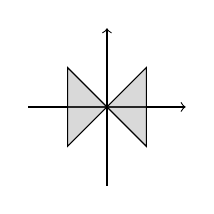
\begin{tikzpicture}
 \draw[->] (0,-1) -- (0,1);
 \draw[->] (-1,0) -- (1,0);
 \draw[fill=gray, fill opacity=0.3] (0,0) -- (0.5,-0.5) -- (0.5,0.5) -- (0,0) -- (-0.5,0.5) -- (-0.5,-0.5) -- cycle;
\end{tikzpicture}\]
\end{example}

\begin{definition}
 Let $R$ be a normed field and let $\mathbb{V}$ be a topological $R$-vector space. We say that $\mathbb{V}$ is \emph{locally convex} iff every $x\in \mathbb{V}$ admits a local basis consisting of disks at $x$.
 Since the topology of $\mathbb{V}$ is necessarily translation invariant,
 it is equivalent to only ask that $0$ has such a local basis.
\end{definition}

The main result is the following:

\begin{proposition}\label{prop:mainLCTVS}
 Let $\mathbb{V}$ be a locally convex topological $\R$-vector space (where $\R$ is endowed with its usual absolute value and the induced topology by it).
 Fix $x\in\mathbb{V}$, a neighbourhood $V\subseteq\mathbb{V}$ of $x$ and $f:V\to \R\cup\set{+\infty,-\infty}$.
 If $V$ is convex, $f$ is concave and lower bounded by a finite constant $K$, then $f$ is continuous at $x$ (w.r.t.\ the subspace topology on $V$).
\end{proposition}
\begin{proof}
 Since $V$ is a neighbourhood of $x$, $x$ admits an open neighbourhood $U\subseteq V$, and by local convexity of $\mathbb{V}$ there is a (non necessary open) disk $D\subseteq U$ at $x$.
 Now fix $\eps\in(0,1)$ and $r,s\in \R$ with $0\leq r\leq\eps$, $s=1-r$.
 Fix also $w\in D$.
 By the convexity of $D$ we have $sx+rw\in D$, and thus the convexity of $f$ entails that:
 \[
  f(sx+rw)\geq s f(x) + r f(w) \geq s f(x) + r K = (1-r)f(x) + r K
 \]
that is,
 \[
  f(x)-f(sx+rw)\leq r (f(x)-K).
 \]
 Now remark that $x=\dfrac{1}{s+2r}(sx+rw)+\dfrac{r}{s+2r}(2x-w)$, where $\dfrac{1}{s+2r}+\dfrac{r}{s+2r}=1$, $\dfrac{1}{s+2r}<1$ and $2x-w\in D$ (because $D$ is a disk at $x$).
 Therefore by the convexity of $f$ we have:
 \[
  f(x)\geq \dfrac{1}{s+2r}f(sx+rw)+\dfrac{r}{s+2r}f(2x-w)\geq \dfrac{1}{s+2r}(f(sx+rw)+rK)
 \]
 that is,
 \[
  f(sx+rw)-f(x)\leq r(f(x)-K).
 \]
 We have thus shown that $\mid f(sx+rw)-f(x)\mid\leq r(f(x)-K)$ for all $w\in D$.
 Since this holds also for all $\eps\in(0,1)$, and due to the choice of $r,s$, the points of shape $sx+rw$ span $D$ when $w$ spans $D$ and $\eps$ spans $(0,1)$.
 That is, we have shown that $\mid f(w)-f(x)\mid\leq r(f(x)-K)$ for all $w\in W$.
 Since $f(x)-K\geq 0$ and $r\leq \eps$, we have that $\exists\lim\limits_{w\to x} f(w)=f(x)$.
\end{proof}

Now we show how to apply this argument to our tropical case $\Lawv^X$, which is \emph{not} a LCTVS (because it is not a vector space).

First, we have:

\begin{corollary}\label{cor:cont}
 Let $f:({\R}_{> 0}^X,\supnorm{.}) \to (\overline\R_{\geq 0},\absv .)$ and $x\in {\R}_{> 0}^X$.
 If there is a convex neighbourhood $V\subseteq \overline{\R}_{> 0}^X$ of $x$ s.t.\ $f_{\lVert V}$ is concave, then $f$ is continuous at $x$.
\end{corollary}
\begin{proof}
 The $\R$-vector space $\R^X$ is topological w.r.t.\ the topology $\tau_\infty$ induced on it by the norm $\lVert .\lVert_\infty$, and it is clearly locally convex.
 Call $\tau^+_\infty$ the topology induced by $\supnorm{.}$ on ${\R}_{> 0}^X$.
 It is clear that it coincides with $\tau^+_\infty$.
 Since moreover ${\R}_{> 0}^X$ is open in $(\R^X,\tau_\infty)$, the neighbourhood $V$ of $x$ in $({\R}_{> 0}^X,\supnorm{.})$ is also a neighbourhood of $x$ in $(\R^X,\tau_\infty)$.
 We can therefore apply Proposition~\ref{prop:mainLCTVS} to $f_{\lVert V}$ (which is lower bounded by $0$ by definition of $f$) and obtain that $f_{\lVert V}$ is continuous at $x$ w.r.t.\ the subspace topology $\tau_V$ induced by $\tau_\infty$ on $V$.
 But since $V$ is contained in ${\R}_{> 0}^X$, the topology $\tau_V$ coincides with the subspace topology induced on $V$ by $\tau^+_\infty$.
 So $f$ is continuous at $x$ w.r.t.\ $\tau^+_\infty$.
\end{proof}

One may wonder if the same proof as above makes it possible to state the previous corollary replacing ${\R}_{> 0}^X$ with $\R_{\geq 0}^X$ (so, in particular, taking $x\in\R_{\geq 0}^X$).
This is not possible because in the proof we crucially use that $\R_{> 0}^X$ is open in $(\R^X,\tau_\infty)$, which is not the case of $\R_{\geq 0}^X$.
In fact, this allowed us to say that $V$ is a neighbourhood of $x$ in $(\R^X,\tau_\infty)$, and therefore to be able to apply Proposition~\ref{prop:mainLCTVS}.
Taking $\R_{\geq 0}^X$ instead, this is in general not true: we could have a neighbourhood of $x$ w.r.t.\ the subspace topology on $\R_{\geq 0}^X$ induced by $\tau_\infty$, which does not contain any open neighbourhood of $x$ w.r.t.\ $\tau_\infty$ (i.e. it is not a neighbourhood w.r.t.\ $\tau_\infty$).

\begin{example}
 An example of a neighbourhood of $x$ w.r.t.\ the subspace topology on $\R_{\geq 0}^X$ induced by $\tau_\infty$, which is not a neighbourhood w.r.t.\ $\tau_\infty$.
 \[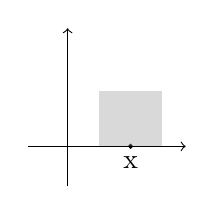
\begin{tikzpicture}
 \draw[->] (0,-0.5) -- (0,1.5);
 \draw[->] (-0.5,0) -- (1.5,0);
 \filldraw[black] (0.8,0) circle (0.7pt) node[anchor=north]{x};
 \fill[fill=gray, fill opacity=0.3] (0.4,0) -- (1.2,0) -- (1.2,0.7) -- (0.4,0.7) -- (0.4,0) -- cycle;
\end{tikzpicture}\]
\end{example}

Finally we have the desired result Theorem~\ref{thm:cont}:

\begin{theorem}[Theorem~\ref{thm:cont}]
 Tropical Laurent series $f:({\R}_{\geq 0}^X,\supnorm .) \to (\overline\R_{\geq 0},\absv .)$ are continuous on ${\R}_{> 0}^X$ w.r.t.\ the norm $\norm{\cdot}_\infty$.
\end{theorem}
\begin{proof}
 We know that tLs's are concave on all their domain.
 Therefore the result immediate follows by Corollary \ref{cor:cont}, since the topology induced by $\supnorm{.}$ on ${\R}_{> 0}^X$ coincides with the subspace topology induced by $({\R}_{\geq 0}^X,\supnorm .)$ on it.
\end{proof}

Due to the previous discussion about the impossibility of stating Corollary \ref{cor:cont} in the case where one of the coordinates of $x$ is $0$, the continuity of tropical functions on the hyperplanes $\mathcal H_a:=\set{x\in {\R}_{\geq 0}^X \mid x_a=0}$, for $a\in X$, must be treated separately.
Similarly, the continuity at points with infinite coordinates must be treated separately as well.
We left it for future investigations.

\begin{remark}
 We formulated the main argument (Proposition~\ref{prop:mainLCTVS}) in the general setting of LCTVS's.
We did so just to show that it is actually a general argument, but we could have placed ourselves already in a more particular setting of our interest and carry on the proof.
For instance, Theorem~\ref{thmTLSlocLip} will be proved by refining this kind of argument (Lemma~\ref{lm:mainLip}), but not in the setting of LCTVS.
\end{remark} 

%\newpage

\begin{definition}
 An \emph{$\overline{\R}_{\geq 0}$-cone} is a commutative $\overline{\R}_{\geq 0}$-semimodule with cancellative addition\footnote{I.e.: $x+y=x+y' \Rightarrow y=y'$.}.
\end{definition}

In [Selinger] cones are required to also have ``strict addition'', meaning that $x+y=0 \Rightarrow x=y=0$.
We do not add this requirement since it will automatic hold when considering normed cones.

\begin{remark}
 The addition of a cone $P$ (which forms a commutative monoid) turns $P$ into a poset by setting:
 \[
  x \leq y \textit{ iff } y=x+z \textit{, for some }z\in P.
 \]
 By the cancellative property, when such $z$ exists it is unique, and we denote it by $y-x$.
 Such order is called the \emph{cone-order} on $P$.
\end{remark}

\begin{definition}
 A \emph{normed $\overline{\R}_{\geq 0}$-cone} is the data of a $\overline{\R}_{\geq 0}$-cone together with a $\leq$-monotone\footnote{I.e.: $x\leq y \Rightarrow \norm{x}\leq \norm y$. Remark that requiring this property (for all $x,y$) is equivalent to requiring that $\norm{x}\leq \norm{x+y}$ for all $x,y$.} norm\footnote{A \emph{norm} on a $\overline{\R}_{\geq 0}$-abstract cone $P$ is a map $\norm{.}:P\to \overline{\R}$ satisfying the usual axioms of norms:
 $\norm x \geq 0$, $\norm x = 0 \Rightarrow x=0$, $\norm{rx}=r\norm x$ and $\norm{x+y}\leq \norm x + \norm y$.} on it.
\end{definition}

In [Ehrhard-Pagani-Tasson, Crubillie] a normed $\overline{\R}_{\geq 0}$-cone is simply called a cone.

Remark that in a normed $\overline{\R}_{\geq 0}$-cone, by monotonicity of the norm, we have: $\norm{x+y}=0 \Rightarrow x=y=0$.
Therefore, as already mentioned, in a normed cone we have: 
$x+y=0 \Rightarrow \norm{x+y}=0 \Rightarrow x=y=0$, that is, addition is strict.

\begin{example}
 $\overline{\R}_{\geq 0}^X$ is a normed cone with the norm $\supnorm{x}:=\sup\limits_{a\in X} x_a\in \overline{\R}_{\geq 0}$.
\end{example}

\begin{remark}
 The cone-order on $\overline{\R}_{\geq 0}^X$ is the pointwise usual order on $\overline{\R}_{\geq 0}$.
 
 Remark also that tropical functions have no reason to be linear nor sublinear.
\end{remark}

\begin{remark}\label{rmk:tropMonot}
 Tropical functions are monotone w.r.t.\ to the cone order on its domain and codomain.
 This is clear, using the definition of tropical functions, because $\mu x\leq \mu y$ if $x\leq y$.
\end{remark}

\begin{remark}
 The cone-order on $\overline{\R}_{\geq 0}^X$ makes it into a dcpo with least element $0$.
\end{remark}

The following is a usual domain theoretical lemma.

\begin{lemma}\label{lm:sup=sup}
 Let $P$ be a poset and $X, I$ sets. Fix the pointwise order on $P^X$.
 \begin{enumerate}
  \item Let $x^i\in P^X$ for $i\in I$.
  If $\bigvee\limits_{i\in I} x^i$ exists $P^X$, then $\bigvee\limits_{i\in I} x^i_a$ exists in $P$ for all $a\in X$, and we have: $\bigvee\limits_{i\in I} x^i_a=\left(\bigvee\limits_{i\in I} x^i\right)_a$.
 \item Let $x^i_a\in P$ for $i\in I,a\in X$.
  If $\bigvee\limits_{i\in I} x^i_a$ exists $P$ for all $a\in X$, then $\bigvee\limits_{i\in I} x^i$ exists in $P^X$, and we have: $\left(\bigvee\limits_{i\in I} x^i\right)_a=\bigvee\limits_{i\in I} x^i_a$.
 \end{enumerate}
\end{lemma}

A \emph{directed net} in a poset $P$ with indices in a set $I$ is a function $s:I\to P$, denoted by $(s_i)_{i\in I}$, s.t.\ its image is directed.
We say that a directed net in $P$ \emph{admits a sup} iff its image admits a sup in $P$.
We say that a directed net $s$ in a normed cone is \emph{bounded} iff the set $\set{\norm{s_i}\,\mid i\in I}$ is bounded in $\R_{\geq 0}$.

Remember the definition of Scott-continuity:

\begin{definition}
 A function $f:P\to P'$ between posets is \emph{Scott-continuous} iff for all directed net $(s_i)_i$ in $P$ admitting a sup, we have $\exists \bigvee\limits_i f(s_i) = f(\bigvee\limits_i s_i)$ in $P'$. 
\end{definition}

The fundamental result in order to prove Theorem~\ref{thm:ScottCont} is the following, taken from [Selinger].

\begin{proposition}\label{prop:infsup}
 Let $P$ be a normed $\overline{\R}_{\geq 0}$-cone s.t.\ every bounded directed net in $P$ admits a sup.
 Let $(v_i)_{i\in I}$ be a directed net in $P$ with an upper bound $v\in P$.
 Then $\exists\bigvee\limits_{i\in I} v_i \in P$ and, if $\inf\limits_{i\in I} \norm{v-v_i} =0$, one has: $\bigvee\limits_{i\in I} v_i = v$.
\end{proposition}
\begin{proof}
 Remark that $v-v_i$ exists in $P$ by hypothesis and so does $\bigvee\limits_{i\in I} v_i$, thanks to the monotonicity of the norm.
 Now, since $v\geq v_i$ for all $i$, we have that $v\geq \bigvee\limits_{i\in I} v_i$, and so $v-\bigvee\limits_{i\in I} v_i$ exists in $P$.
 Fix $i\in I$.
 Since $v_i\leq \bigvee\limits_{i\in I} v_i$, then $v-\bigvee\limits_{i\in I} v_i\leq v-v_i$ and, by monotonicity of the norm, $\norm{v-\bigvee\limits_{i\in I} v_i}\leq \norm{v-v_i}$.
 Since this holds for all $i\in I$, we have:
 $0\leq \norm{v-\bigvee\limits_{i\in I} v_i}\leq \inf\limits_{i\in I} \norm{v-v_i}=0$, where the last equality holds by hypothesis.
 Thus $\norm{v-\bigvee\limits_{i\in I} v_i}=0$, i.e.\ $v=\bigvee\limits_{i\in I} v_i$.
\end{proof}

\begin{definition}
 A normed $\overline{\R}_{\geq 0}$-cone $P$ is \emph{Scott-complete} iff its norm is Scott-continuous (where the codomain $\overline\R_{\geq 0}$ is endowed with its usual order) and every bounded directed net in $P$ admits a sup.
 This is equivalent to asking that its closed unit ball is a dcpo.
\end{definition}

\begin{proposition}
 The normed cone $\overline{\R}_{\geq 0}^X$ is Scott-complete.
\end{proposition}
\begin{proof}
 $\overline{\R}_{\geq 0}^X$ being a dcpo, all the existences of sup's that we should check do automatically hold, so we only have to show that $\bigvee$ and $\supnorm{.}$ commute:
 $\supnorm{\bigvee\limits_i x_i}=
 \sup\limits_a\, \sup\limits_i\, (x_i)_a =
 \sup\limits_i\, \sup\limits_a\, (x_i)_a =
 \bigvee\limits_i \supnorm{x_i}$.
\end{proof}

%Let us set $\infty_b$ to be the hyper-semi-plane $\set{y\in\overline{\R}^Y_{\geq 0}\mid y_b=+\infty}$ and $\set{f<<+\infty}:=\bigcup\limits_{b\in Y} f^{-1}\infty_b$.

%\begin{remark}\label{rmk:R-f<<oo}
%Let $f:\overline{\R}^X_{\geq 0}\to\overline{\R}^Y_{\geq 0}$ be tropical.
%Then, $\R^X_{> 0}-\set{f<<+\infty}$ is a dcpo (w.r.t.\ the usual order, that is, its cone order).
%In order to see this, it is enough to show that, for any $b\in Y$ and for any directed net $(x^i)_i$ in $\R^X_{> 0}$ s.t.\ $f(x^i)_b<+\infty$ for all $i$, we have $f(\bigvee\limits_i x^i)_b<+\infty$ (where the sup is taken in $\R^X_{> 0}$).
%Such property holds because otherwise it is easy to see that $f$ would be discontinuous at the point $\bigvee\limits_i x^i\in\R^X_{> 0}$ w.r.t.\ the topology\footnote{Remark that this argument would not be possible using Scott-continuity instead. Indeed, it could well be that $f(\bigvee\limits_i x^i)_b=\bigvee\limits_i f(x^i)_b=+\infty$ while $f(x^i)_b<+\infty$ for all $i$.} induced by $\supnorm{.}$.
%This contradicts Corollary \ref{cor:tropCont}.
%\end{remark}

\begin{proposition}
 All tropical functions $f:\overline{\R}^X_{\geq 0}\to\overline{\R}^Y_{\geq 0}$ are Scott-continuous on $\R^X_{> 0}$ w.r.t.\ the cone-orders on its domain and codomain.
\end{proposition}
\begin{proof}
 Let $(x_i)_i$ a directed net in $\R^X_{> 0}$ s.t.\ $\bigvee\limits_i x^i$ exists in $\R^X_{> 0}$.
 Then $\inf\limits_i \supnorm{\bigvee\limits_i x^i - x^i} =0$, where $\bigvee\limits_i x^i - x^i$ exists because $\bigvee\limits_i x^i \geq x^i$ for all $i$.
 Since $f$ is $\supnorm{.}$-continuous on $\R^X_{> 0}$ (Corollary \ref{cor:tropCont}), then $\inf\limits_i \supnorm{f(\bigvee\limits_i x^i) - f(x^i)} =0$, where $f(\bigvee\limits_i x^i) - f(x^i)$ exists because $f(\bigvee\limits_i x^i) \geq f(x^i)$ for all $i$ being $f$ monotone (Remark \ref{rmk:tropMonot}).
 We can therefore apply Proposition \ref{prop:infsup} to the directed net $(f(x^i))_i$ in $\overline{\R}^Y_{\geq 0}$, obtaining that $\bigvee\limits_i f(x^i)$ exists in $\overline{\R}^Y_{\geq 0}$ and it coincides with $f(\bigvee\limits_i x^i)$.
\end{proof}

%\begin{remark}
%By looking at the definition of tropical functions, for $f$ tropical we have that: if $x,x'\in\R^X_{> 0}-\set{f<<+\infty}$ and $r\in\R_{> 0}$, then $x+x',rx\in\R^X_{> 0}-\set{f<<+\infty}$.
%That is, $\R^X_{> 0}-\set{f<<+\infty}$ is a $\R_{>0}$-cone.
%It is clearly still Scott-complete.
%\end{remark}

In the main paper we mention that $\R_{\geq0}^X$ is a Scott-complete dcpo.
We did not state it as a theorem because it follows from standard and well-known domain theoretical considerations.
Let us prove it here anyway.

Recall the definition of Scott-complete dcpo:

\begin{definition}
 Let $P$ be a dcpo and define a relation by: $x<<y$ iff for all directed $D\subseteq P$, if $y\leq \bigvee D$, then $x\leq d$, for some $d\in D$.
 Call $\twoheaddownarrow y:=\set{x\in P\mid x<<y}$.
 A dcpo $P$ is \emph{Scott-continuous} iff $\twoheaddownarrow x$ is directed and $x=\bigvee\twoheaddownarrow x$ for all $x\in P$.
\end{definition}

\begin{remark}
 In any dcpo we have: $\twoheaddownarrow x \subseteq \downarrow x$.
 This immediately follows by considering the directed set $\set{x}$.
\end{remark}

\begin{lemma}\label{lm:<<dir}
 In $\overline{\R}_{\geq 0}^X$, every set $\twoheaddownarrow x$ is directed.
\end{lemma}
\begin{proof}
 It is immediate that $0\in\twoheaddownarrow x$, so it is non-empty.
 Now let $y,y' << x$.
 Since we are in $\overline{\R}_{\geq 0}^X$, there is $y\vee y'\in\overline{\R}_{\geq 0}^X$.
 So we only have to show that $y\vee y'<<x$.
 For that, let $D$ be a directed set in $\overline{\R}_{\geq 0}^X$ s.t.\ $x\leq\bigvee D$.
 Since $y,y' << x$ we find $d,d'\in D$ s.t.\ $y\leq d$, $y'\leq d'$.
 Since $D$ is directed, there is $\hat d\in D$ s.t.\ $y\leq d\leq \hat d\geq d'\geq y'$.
 But then, by definition of sup, it must be $\hat d\geq y\vee y'$ and we are done.
\end{proof}

\begin{remark}
 The following is a known property (that we will not use):
 let $P$ be a complete normed cone which is a dcpo w.r.t.\ its cone-order. Then $P$ is Scott-continuous as a dcpo iff its closed unit ball is Scott-continuous as a dcpo.
\end{remark}

\begin{remark}\label{rmk:<<R}
 Consider $\overline{\R}_{\geq 0}$ with its usual order (which coincides with its cone-order).
 It is easily seen (and well known) that $y<<x$ iff either $y=0$ or $y<x$.
 This immediately implies that $\overline{\R}_{\geq 0}$ is Scott-continuous, since $x=\sup\limits_{y<x} y$.
\end{remark}

\begin{lemma}\label{lm:<<RX}
 Let $x,y\in \overline{\R}_{\geq 0}^X$ (considered as a dcpo with its cone order, which is the pointwise one). Fix $a\in X$.
 If $y_a<<x_a$ and $y_c=0$ for all $c\neq a$, then $y<<x$.
\end{lemma}
\begin{proof}
 Towards a contradiction, assume that there is a directed set $D$ in $\overline{\R}_{\geq 0}^X$ with $x\leq\bigvee D$ and s.t.\ $y\not\leq d$ for all $d\in D$.
 Call $D_a:=\set{d_a\mid d\in D}$ and remark that it is directed, because $D$ is.
 Also, by Lemma \ref{lm:sup=sup}, $\bigvee D_a = \left(\bigvee D\right)_a$.
 Therefore from $y_a<<x_a\leq \bigvee D_a$ we obtain a $d\in D$ s.t.\ $y_a\leq d_a$.
 By the absurd hypothesis we have $y\not\leq d$, so there must be $c\in X$ s.t.\ $y_c\not\leq d_c$, i.e. (because real numbers are totally ordered) $y_c>d_c$.
 Therefore it must be $c\neq a$.
 But then we have $0=y_c>d_c\geq 0$, contradiction.
\end{proof}

\begin{lemma}\label{lm:<<_a}
 In $\overline{\R}_{\geq 0}^X$ we have:
 if $y<<x$ then $y_a<< x_a$ for all $a\in X$.
\end{lemma}
\begin{proof}
 Fix $a\in X$.
 Let $D$ directed set in $\overline{\R}_{\geq 0}$ s.t.\ $x_a\leq\bigvee D$.
 We look for a $d\in D$ s.t.\ $y_a\leq d$.
 For $d\in D$, let $x^{a,d}\in\overline{\R}_{\geq 0}^X$ defined by $x^{a,d}_c:=x_c$ if $c\neq a$ and $x^{a,d}_a:=d$.
 Let $D^x_a:=\set{x^{a,d}\mid d\in D}$.
 By Lemma \ref{lm:sup=sup} $D^x_a$ admits sup in $\overline{\R}_{\geq 0}^X$ and it is $(\bigvee D^x_a)_c=x_c$ if $c\neq a$ and $(\bigvee D^x_a)_a=\bigvee D$.
 Hence, $x\leq \bigvee D^x_a$.
 If we prove that $D^x_a$ is directed, we are done: indeed, since $y<<x$, there is $d\in D$ s.t.\ $y\leq x^{a,d}$ and thus, in particular, $y_a\leq x^{a,d}_a=d$.
 Let us finally prove that $D^x_a$ is directed: it is clearly non-empty, since $D$ is.
 Let now $d,d'\in D$.
 We want to show that there is $\hat d\in D$ s.t.\ $x^{a,d}\leq x^{a,\hat d}\geq x^{a,d'}$.
 But since $D$ is directed, there is $\hat d\in D$ s.t.\ $d\leq \hat d\geq d'$, and therefore $x^{a,d}_c=x_c= x^{a,\hat d}_c =x_c=x^{a,d'}_c$ for all $c\neq a$, and $x^{a,d}_a=d\leq \hat d=x^{a,\hat d}_a=\hat d \geq d'=x^{a,d'}_a$.
\end{proof}

\begin{lemma}\label{rmk:sup_a=sup_a}
In $\overline{\R}_{\geq 0}^X$ we have:
$\bigvee\limits_{y<<x_a} y = \bigvee\limits_{y<<x} y_a$.
\end{lemma}
\begin{proof}
 If we show that $\twoheaddownarrow x_a = \set{y_a\mid y\in\twoheaddownarrow x}$, then we are done because in the statement we are taking their sup's.
 The inclusion ($\supseteq$) immediately follows from Lemma \ref{lm:<<_a}. For ($\subseteq$), let $d<< x_a$.
 Then the $y\in \overline{\R}_{\geq 0}^X$ defined by $y_c:=0$ if $c\neq a$ and $y_a:=d$, is s.t.\ $y\in\twoheaddownarrow x$ by Lemma \ref{lm:<<RX}.
 Thus, $d\in \set{y_a\mid y\in\twoheaddownarrow x}$.
\end{proof}


\begin{corollary}
 The dcpo $\overline{\R}_{\geq 0}^X$ is Scott-continuous.
\end{corollary}
\begin{proof}
 The fact that $\twoheaddownarrow x$ is directed is given by Lemma \ref{lm:<<dir}. The fact that $x=\bigvee \twoheaddownarrow x$ is given by the following equalities:
 $x_a=\bigvee\limits_{y<<x_a} y = \bigvee\limits_{y<<x} y_a = \left(\bigvee\limits_{y<<x} y\right)_a=\left(\bigvee \twoheaddownarrow x\right)_a$.
 The first equality follows from Remark \ref{rmk:<<R}, the second one from Lemma \ref{rmk:sup_a=sup_a}, the third one from Lemma \ref{lm:sup=sup}.
\end{proof}

\newpage



\subsubsection{Lipschitz continuity}





  We need a first, preliminary, lemma:
\begin{lemma}\label{lemma:inf}
Let $u,v: I\to Q$ and suppose $|u(i)-v(i)|\leq \delta$, for all $i\in I$.
Then $|\inf_{i\in I}u(i)- \inf_{i\in I}v(i)|\leq \delta$. 
\end{lemma}
\begin{proof}
Let $A=\inf_{i\in I}u(i)$ and $B=\inf_{i\in I}v(i)$ and suppose $A\geq B$. 
Suppose by way of contradiction $|A-B|> \delta$; then there exists $i\in I$ such that 
$v(i)<A$ and $|A-v(i)|> \delta$. Indeed, otherwise we would have $|A-B|= \sup\{ |A-v(i)|\mid v(i)\leq A\}\leq \delta$. 
Now, from $|A-v(i)|> \delta$ and $v(i)< A$ we deduce that $|u(j)-v(i)|> \delta$ for all $j\in I$, and thus in particular that $|u(i)-v(i)|>\delta$, against the assumption. We conclude then $|A-B| \leq \delta$.
In case $B\geq A$, we can argue in a similar way. 
\end{proof}



\begin{proposition}\label{prop:troplinear}
All tropical linear functions $f: \Lawv^{X}\to \Lawv^{Y}$ are non-expansive.  
\end{proposition}
\begin{proof}
%All functions of the form $f_{\theta,\eta}(x)_{b}= \theta(b)+x_{\eta(b)}$, where $\theta:Y \to \Lawv$ and $\eta:Y\to X$, are non-expansive: indeed $|f_{\theta,\eta}(x)_{b}-f_{\theta,\eta}(y)_{b}|= |\theta(b)+x_{\eta(b)}-\theta(b)-y_{\eta(b)}|=
%|x_{\eta(b)}-y_{\eta(b)}|\leq \norm{x-y}_{\infty}$.
Let $f(x)_{b}=\inf_{a}\{\widehat f_{a,b}+x_{a}\}$.
For all $a\in X$ we have that 
$|(\widehat f_{a,b}+x_{a})- (\widehat f_{a,b}+y_{a})|=
|x_{a}-y_{a}|\leq \norm{x-y}_{\infty}$. Using Lemma \ref{lemma:inf}, we deduce then 
$|f(x)_{b}-f(y)_{b}|=|\inf_{a}\{\widehat f_{a,b}+x_{a}\}-
\inf_{a}\{\widehat f_{a,b}+y_{a}\}|\leq \norm{x-y}_{\infty}$.
\end{proof}






\begin{lemma}\label{lm:mainLip}
Let $f: [0,\infty)^{X}\to Q$ be concave, monotone increasing, and continuous.  
Let $ x \neq  y  \in [0,\infty)^{X}$, with $\| x - y  \|_{\infty}<\infty$, and let $S( x ,  y  )=\{ \alpha x  + (1-\alpha) y  \mid \alpha \in [0,1]\}$ be the segment generated by $ x $ and $ y  $. 
Then $f$ is Lipschitz-continuous over $S( x ,  y  )$.

\end{lemma}
\begin{proof}
Let us prove the lemma under the assumption that for all $a\in X$, $ y  _{a}- x _{a}\geq 1$. From the fact that the claim holds under the assumption, we can deduce the claim of the lemma:
indeed for $\alpha\in (0,1)$ large enough we have that $ y  ':= \frac{ y  -\alpha x }{1-\alpha}$ is such that $ y  \in S( x ,  y  ')$ (and thus $S( x ,  y  )\subseteq S( x ,  y  ')$) and 
$ y  '_{a}- x _{a}\geq 1$. Hence from our proof we deduce that $f$ is Lipschitz-continuous over $S( x ,  y  ')$, and thus a fortiori over $S( x ,  y  )$ too.


Since $f$ is continuous over $[0,\infty)^{X}$ and $S( x ,  y  )$ is compact, $f$ admits a maximum $\mathrm{MAX}$ over $S( x ,  y  )$.
For all $ z  <  z  '\in S( x ,  y  )$, let $M( z  ,  z  ')\in Q^{X}$ be defined by
$$
M( z  ,  z  ')_{a}= \frac{f( z  ')-f( z  )}{ z  '_{a}- z  _{a}}
$$
Observe that
\begin{align*}
M( x ,  y  )_{a} & = \frac{f( y  )-f( x )}{ y  _{a}- x _{a}} \leq 
f( y  )-f( x ) \leq \mathrm{MAX}
\end{align*}
using the fact that $ y  _{a}- x _{a}\geq 1$. 

We now claim that $M( z  ,  z  ')$ is contravariant in both $ z  $ and $ z  '$. 
Indeed suppose $ z  \leq  z  '' <  z  '$, so that $ z  = \lambda  z  ' +(1-\lambda) z  ''$ for some $\lambda \in (0,1)$. Then, using the fact that $f$ is concave, we have 
\begin{align*}
M( z  ,  z  ')_{a}&=\frac{f( z  ')-f(\lambda  x  +(1-\lambda) z  '')}{ z  '_{a}-\lambda  x _{a} -(1-\lambda) z  ''_{a}} \\
&
\geq 
\frac{f( z  ')-\lambda f( z  ') -(1-\lambda)f( z  '')}{ z  '_{a}-\lambda  z  '_{a} -(1-\lambda) z  ''_{a}} \\
&
= 
\frac{(1-\lambda)(f( z  ')-f( z  ''))}{(1-\lambda ) z  '_{a}- z  ''_{a}} =M( z  '',  z  ')
\end{align*}
In a similar way it is shown that for $ z   <  z  ''\leq  z  '$, $M( z  , z  ')\leq M( z  ,  z  '')$. 

Therefore, for all $ z   <  z  '\in S( x ,  y  )$, we have that $M( z  ,  z  ')_{a} \leq M( x ,  z  ')_{a} \leq M( x ,  y  )_{a} \leq \mathrm{MAX}$. 
From this, using the fact that $f$ is monotone increasing, we deduce that 
$|f( z  ')-f( z  )|=f( z  ')-f( z  ) \leq \mathrm{MAX}\cdot | z  '_{a}- z  _{a}|
$ and thus that 
$$|f( z  ')-f( z  )|\leq \mathrm{MAX}\cdot \| z  '- z  \|_{\infty}$$
that is, that $f$ is $\mathrm{MAX}$-Lipschitz over $S( x ,  y  )$. 
\end{proof}

\begin{proposition}
Let $f: [0,\infty)^{X}\to Q$ be concave, monotone increasing, and continuous.  
For all $\epsilon \in (0,\infty)$ and $ x \in [0,\infty)^{X}$, $f$ is Lipschitz-continuous over the open ball $B( x , \epsilon)$.
\end{proposition}
\begin{proof}
Let $\mathrm{MAX}$ indicate the maximum of $f$ over $B( x , \epsilon)$. 
Let $ y  ,  z  \in B( x , \epsilon)$; then $\| y  - z  \|_{\infty}\leq 2\epsilon < \infty$, so by the lemma above $f$ is $K$-Lipschitz over the segment $S( y  ,  z  )$ for some $K\leq \mathrm{MAX}$, so we deduce $|f( y  )-f( z  )|\leq \mathrm{MAX}\cdot \| y  - z  \|_{\infty}$.
\end{proof}

\begin{theorem}[local Lipschitz-continuity]
Let $f: [0,\infty)^{X}\to Q$ be concave, monotone increasing, and continuous.  
Then $f$ is locally Lipschitz-continuous.
\end{theorem}
\begin{proof}
For all $ x \in [0,\infty)^{X}$, $f$ is Lipschitz-continuous over the open set $B( x , 1)$.
\end{proof}



\subsubsection{Characterizations of the functional metric }



  \begin{proposition}\label{prop:functionalmetric}
For all maps $f,g: Q\langle X\rangle\to Q\langle Y\rangle$,  
$$
  \|\widehat f- \widehat g\|_{\infty}=
  \sup\{\|f( x )- g( x )\|_{\infty} \mid  x \in Q\langle X\rangle\}
$$

\end{proposition}
  
%
%\begin{lemma}
%Let $f,g\in\mathsf{Trop}(1,1)$ (i.e.~$f,g:Q\to Q$), and suppose for all $n\in \BB N$, 
%$|\widehat f_{n}-\widehat g_{n}|\leq \delta$. Then for all $x\in Q$, $|f(x)-g(x)|\leq \delta$.
%
%\end{lemma}
%\begin{proof}
%$|f(x)-g(x)|= |( \inf_{n}nx+\widehat f_{n})- (\inf_{n}nx+\widehat g_{n})|$. 
%Since $|nx+\widehat f_{n} - nx -\widehat g_{n}|= |\widehat f_{n}-\widehat g_{n}|\leq \delta$, by the Lemma above we conclude $|f(x)-g(x)|\leq \delta$. 
%\end{proof}



  
  \begin{proof}[Proof of Proposition \ref{prop:functionalmetric}]
For one side, suppose for all $\mu\in \C  M_{\mathrm{fin}}(X),b\in Y$, 
$|\widehat f_{\mu,b}-\widehat g_{\mu,b}|\leq \delta$. Then for all $ x \in Q\langle X\rangle$ and $b\in Y$, $|f( x )(b)-g( x )(b)|\leq \delta$.
Indeed, $|f( x )(b)-g( x )(b)|= |( \inf_{\mu}\mu  x +\widehat f_{\mu,b})- (\inf_{\mu}\mu  x +\widehat g_{\mu,b})|$. 
Since $|\mu  x +\widehat f_{\mu,b} - \mu  x  -\widehat g_{\mu,b}|= |\widehat f_{\mu,b}-\widehat g_{\mu,b}|\leq \delta$, by Lemma \ref{lemma:inf} we conclude $|f( x )(b)-g( x )(b)|\leq \delta$. 


For the other side, suppose for some $\mu\in \C M_{\mathrm f}(X)$ and $b\in Y$, $|\widehat f_{\mu,b}-\widehat g_{\mu,b}|> \epsilon$; 
then, by letting $e_{\mu}\in Q\langle !X\rangle$ be the (tropical) characteristic function of $\mu$, we have
 $|f(e_{\mu})({b})-g(e_{\mu})({b})| =
|( \inf_{\mu'}\widehat f_{\mu',b}+ \mu'(e_{\mu}))-
( \inf_{\mu'}\widehat g_{\mu',b}+\mu'(e_{\mu}))|=
|\widehat f_{\mu,b}- \widehat g_{\mu,b}|> \epsilon$, so we deduce that 
$\sup\{\| f( x )- g( x ) \|_{\infty}\mid  x \in Q\langle X\rangle\}> \epsilon$.
\end{proof}


The second characterization relates distances with the Taylor expansion. Let us briefly discuss the latter, first.
For all $f: Q\langle X\rangle \to Q\langle Y\rangle$, let $\delta^{(n)}f:Q\langle X^{n}\rangle \to Q\langle Y\rangle$ indicate the $n$-linear function given by 
$$
\delta^{(n)}f( x ^{n})= D^{(n)}f( x ^{n}, \infty)
$$

Notice that $\widehat{\delta^{(n)}f}\in Q^{X^{n}\times Y}$ satisfies 
$\widehat{\delta^{(n)}f}_{a_{1},\dots, a_{n},b}= \widehat f_{[a_{1},\dots, a_{n}],b}$.
In other words, $\delta^{(n)}f$ precisely captures the behavior of $f$ when applied to multisets of length $n$. Moreover, the full behavior of $f$ can be recovered from the functions $\delta^{(n)}f$ using the Taylor expansion which, in its tropical form, reads as:
\begin{equation*}
f( x )= \inf_{n}\left \{ D^{(n)}f( x ^{n},\infty)\right\}= \inf_{n}\left \{\delta^{(n)}f( x ^{n})\right\}
%\tag{Tropical Taylor}
\end{equation*}





\begin{proposition}\label{prop:taylormetric}
For all $f,g:Q\langle X\rangle \to Q\langle Y\rangle$, 
$$
\| \widehat f-\widehat g\|_{\infty}= \sup_{n}\| \widehat{\delta^{(n)}f} -\widehat{\delta^{(n)}g}\|_{\infty}
$$
\end{proposition}
\begin{proof}
Let us first show that $\| \widehat f-\widehat g\|_{\infty}\leq \epsilon$ implies 
$\| \delta^{(n)}f-\delta^{(n)}g\|_{\infty}\leq\epsilon$, for all $n\in \BB N$. 
Notice that $\widehat{\delta^{(n)}f}\in Q^{X^{n}\times Y}$ satisfies 
$\widehat{\delta^{(n)}f}_{a_{1},\dots, a_{n},b}= \widehat f_{[a_{1},\dots, a_{n}],b}$. Hence 
from $\| \widehat f-\widehat g\|\leq\epsilon$ it follows that for all $\mu=[a_{1},\dots, a_{n}]$ and $b\in Y$, 
$|\widehat f_{\mu,b}- \widehat g_{\mu,b}|\leq \epsilon$, so 
we deduce that $\| \widehat{\delta^{(n)}f}- \widehat{\delta^{(n)}g}\|\leq \epsilon$.

For the converse direction suppose that, for all $n\in \BB N$, $\| \widehat{\delta^{(n)}f}- \widehat{\delta^{(n)}g}\|\leq \epsilon_{n}$. Then, since the family of coefficients $
F_{n,\mu,b}=
( \widehat{\delta^{(n)}f})_{a_{1},\dots, a_{n},b}$ (where $\mu=[a_{1},\dots, a_{n}]$) is in bijection with the coefficients $\widehat f_{\mu,b}$, we deduce that $|\widehat f_{\mu,b}-\widehat g_{\mu,b}|\leq 
\epsilon_{\sharp \mu  }$, and thus that 
$\| \widehat f-\widehat g\|_{\infty}\leq \sup_{n}\epsilon_{n}$. 
\end{proof}

